% Options for packages loaded elsewhere
\PassOptionsToPackage{unicode}{hyperref}
\PassOptionsToPackage{hyphens}{url}
%
\documentclass[
]{article}
\usepackage{amsmath,amssymb}
\usepackage{iftex}
\ifPDFTeX
  \usepackage[T1]{fontenc}
  \usepackage[utf8]{inputenc}
  \usepackage{textcomp} % provide euro and other symbols
\else % if luatex or xetex
  \usepackage{unicode-math} % this also loads fontspec
  \defaultfontfeatures{Scale=MatchLowercase}
  \defaultfontfeatures[\rmfamily]{Ligatures=TeX,Scale=1}
\fi
\usepackage{lmodern}
\ifPDFTeX\else
  % xetex/luatex font selection
\fi
% Use upquote if available, for straight quotes in verbatim environments
\IfFileExists{upquote.sty}{\usepackage{upquote}}{}
\IfFileExists{microtype.sty}{% use microtype if available
  \usepackage[]{microtype}
  \UseMicrotypeSet[protrusion]{basicmath} % disable protrusion for tt fonts
}{}
\makeatletter
\@ifundefined{KOMAClassName}{% if non-KOMA class
  \IfFileExists{parskip.sty}{%
    \usepackage{parskip}
  }{% else
    \setlength{\parindent}{0pt}
    \setlength{\parskip}{6pt plus 2pt minus 1pt}}
}{% if KOMA class
  \KOMAoptions{parskip=half}}
\makeatother
\usepackage{xcolor}
\usepackage[margin=1in]{geometry}
\usepackage{color}
\usepackage{fancyvrb}
\newcommand{\VerbBar}{|}
\newcommand{\VERB}{\Verb[commandchars=\\\{\}]}
\DefineVerbatimEnvironment{Highlighting}{Verbatim}{commandchars=\\\{\}}
% Add ',fontsize=\small' for more characters per line
\usepackage{framed}
\definecolor{shadecolor}{RGB}{248,248,248}
\newenvironment{Shaded}{\begin{snugshade}}{\end{snugshade}}
\newcommand{\AlertTok}[1]{\textcolor[rgb]{0.94,0.16,0.16}{#1}}
\newcommand{\AnnotationTok}[1]{\textcolor[rgb]{0.56,0.35,0.01}{\textbf{\textit{#1}}}}
\newcommand{\AttributeTok}[1]{\textcolor[rgb]{0.13,0.29,0.53}{#1}}
\newcommand{\BaseNTok}[1]{\textcolor[rgb]{0.00,0.00,0.81}{#1}}
\newcommand{\BuiltInTok}[1]{#1}
\newcommand{\CharTok}[1]{\textcolor[rgb]{0.31,0.60,0.02}{#1}}
\newcommand{\CommentTok}[1]{\textcolor[rgb]{0.56,0.35,0.01}{\textit{#1}}}
\newcommand{\CommentVarTok}[1]{\textcolor[rgb]{0.56,0.35,0.01}{\textbf{\textit{#1}}}}
\newcommand{\ConstantTok}[1]{\textcolor[rgb]{0.56,0.35,0.01}{#1}}
\newcommand{\ControlFlowTok}[1]{\textcolor[rgb]{0.13,0.29,0.53}{\textbf{#1}}}
\newcommand{\DataTypeTok}[1]{\textcolor[rgb]{0.13,0.29,0.53}{#1}}
\newcommand{\DecValTok}[1]{\textcolor[rgb]{0.00,0.00,0.81}{#1}}
\newcommand{\DocumentationTok}[1]{\textcolor[rgb]{0.56,0.35,0.01}{\textbf{\textit{#1}}}}
\newcommand{\ErrorTok}[1]{\textcolor[rgb]{0.64,0.00,0.00}{\textbf{#1}}}
\newcommand{\ExtensionTok}[1]{#1}
\newcommand{\FloatTok}[1]{\textcolor[rgb]{0.00,0.00,0.81}{#1}}
\newcommand{\FunctionTok}[1]{\textcolor[rgb]{0.13,0.29,0.53}{\textbf{#1}}}
\newcommand{\ImportTok}[1]{#1}
\newcommand{\InformationTok}[1]{\textcolor[rgb]{0.56,0.35,0.01}{\textbf{\textit{#1}}}}
\newcommand{\KeywordTok}[1]{\textcolor[rgb]{0.13,0.29,0.53}{\textbf{#1}}}
\newcommand{\NormalTok}[1]{#1}
\newcommand{\OperatorTok}[1]{\textcolor[rgb]{0.81,0.36,0.00}{\textbf{#1}}}
\newcommand{\OtherTok}[1]{\textcolor[rgb]{0.56,0.35,0.01}{#1}}
\newcommand{\PreprocessorTok}[1]{\textcolor[rgb]{0.56,0.35,0.01}{\textit{#1}}}
\newcommand{\RegionMarkerTok}[1]{#1}
\newcommand{\SpecialCharTok}[1]{\textcolor[rgb]{0.81,0.36,0.00}{\textbf{#1}}}
\newcommand{\SpecialStringTok}[1]{\textcolor[rgb]{0.31,0.60,0.02}{#1}}
\newcommand{\StringTok}[1]{\textcolor[rgb]{0.31,0.60,0.02}{#1}}
\newcommand{\VariableTok}[1]{\textcolor[rgb]{0.00,0.00,0.00}{#1}}
\newcommand{\VerbatimStringTok}[1]{\textcolor[rgb]{0.31,0.60,0.02}{#1}}
\newcommand{\WarningTok}[1]{\textcolor[rgb]{0.56,0.35,0.01}{\textbf{\textit{#1}}}}
\usepackage{longtable,booktabs,array}
\usepackage{calc} % for calculating minipage widths
% Correct order of tables after \paragraph or \subparagraph
\usepackage{etoolbox}
\makeatletter
\patchcmd\longtable{\par}{\if@noskipsec\mbox{}\fi\par}{}{}
\makeatother
% Allow footnotes in longtable head/foot
\IfFileExists{footnotehyper.sty}{\usepackage{footnotehyper}}{\usepackage{footnote}}
\makesavenoteenv{longtable}
\usepackage{graphicx}
\makeatletter
\def\maxwidth{\ifdim\Gin@nat@width>\linewidth\linewidth\else\Gin@nat@width\fi}
\def\maxheight{\ifdim\Gin@nat@height>\textheight\textheight\else\Gin@nat@height\fi}
\makeatother
% Scale images if necessary, so that they will not overflow the page
% margins by default, and it is still possible to overwrite the defaults
% using explicit options in \includegraphics[width, height, ...]{}
\setkeys{Gin}{width=\maxwidth,height=\maxheight,keepaspectratio}
% Set default figure placement to htbp
\makeatletter
\def\fps@figure{htbp}
\makeatother
\setlength{\emergencystretch}{3em} % prevent overfull lines
\providecommand{\tightlist}{%
  \setlength{\itemsep}{0pt}\setlength{\parskip}{0pt}}
\setcounter{secnumdepth}{-\maxdimen} % remove section numbering
\usepackage{booktabs}
\usepackage{caption}
\usepackage{longtable}
\usepackage{colortbl}
\usepackage{array}
\usepackage{anyfontsize}
\usepackage{multirow}
\ifLuaTeX
  \usepackage{selnolig}  % disable illegal ligatures
\fi
\usepackage{bookmark}
\IfFileExists{xurl.sty}{\usepackage{xurl}}{} % add URL line breaks if available
\urlstyle{same}
\hypersetup{
  pdftitle={Projet de biostatistiques - Ankylostome},
  pdfauthor={Amandine LIAGRE - Florian BUCQUET - Rachid ABDELJABBAR},
  hidelinks,
  pdfcreator={LaTeX via pandoc}}

\title{Projet de biostatistiques - Ankylostome}
\author{Amandine LIAGRE - Florian BUCQUET - Rachid ABDELJABBAR}
\date{03-02-2024}

\begin{document}
\maketitle

{
\setcounter{tocdepth}{3}
\tableofcontents
}
\newpage

\section{Introduction}\label{introduction}

A travers ce projet, nous allons utiliser les données provenant d'une
enquête réalisée sur un échantillon d'individus en Egypte. Plus
particulièrement, nous avons des informations concernant l'infection des
individus par l'ankylostome. En marchant pieds nus, les individus sont
contaminés via les larves des ankylostomes vivant en terre. L'infection
peut aussi se produire via une ingestion d'aliments contaminés par des
larves. Les différents symptômes posibles sont des éruptions et lésions
cutannées aux endroits où les larves ont pénétré la peau, de la fièvre,
des douleurs épigastriques, des diarrhées, de la toux, inflammation de
l'intestin \ldots{} . Dans les cas les plus graves, le malade peut être
victime d'une perte de sang (les larves dans l'intestin se nourrissent
de sang en étant accroché à sa paroi et il en résulte une potentielle
anémie pour le malade), d'insuffisance cardiaque. Il existe des
médicaments antiparasitaires pour traiter cette infection (albendazole,
mébendazole).

L'ankylostome vit particulièrement bien dans la terre et une température
aux alentours des 18°C afin que les oeufs puissent éclore. Les oeufs
d'ankylostomes ont l'allure suivante:

\begin{figure}
\centering
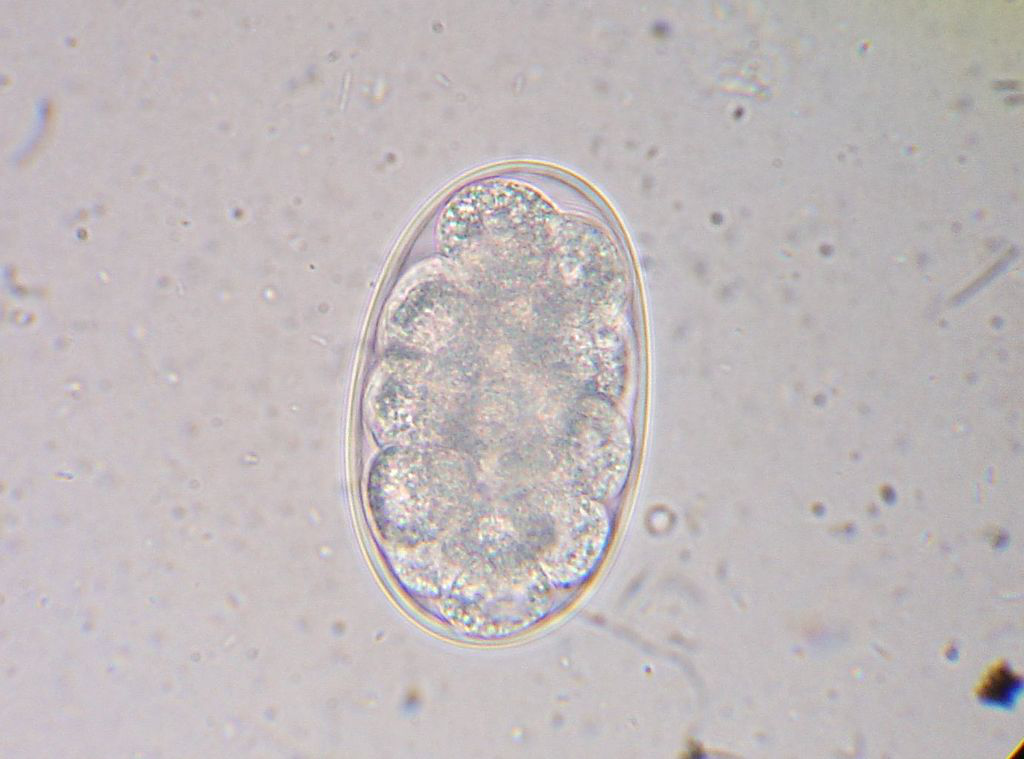
\includegraphics[width=0.4\textwidth,height=\textheight]{egg.png}
\caption{Oeufs d'Ankylostosme, par Joel Mills - CC BY-SA 3.0}
\end{figure}

Et par la suite, deviennent les des vers se propageant vers l'intestin:

\begin{figure}
\centering
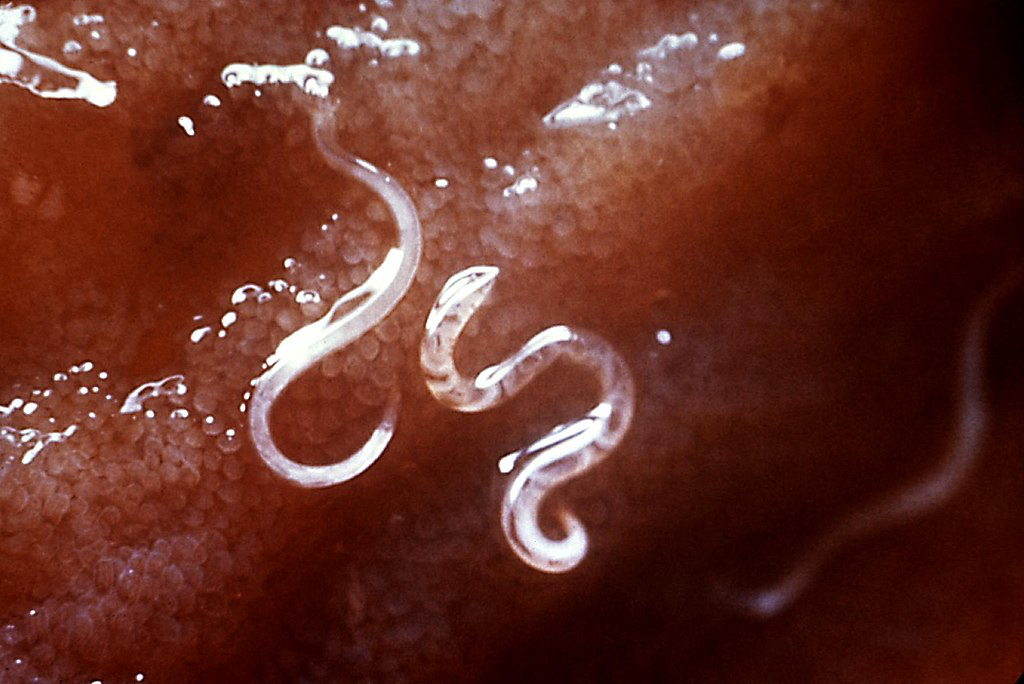
\includegraphics[width=0.4\textwidth,height=\textheight]{Hookworms.png}
\caption{Vers d'Ankylostosme, par CDC's Public Health Image Library}
\end{figure}

Voici le cycle parasitaire de l'ankylostome:

\begin{figure}
\centering
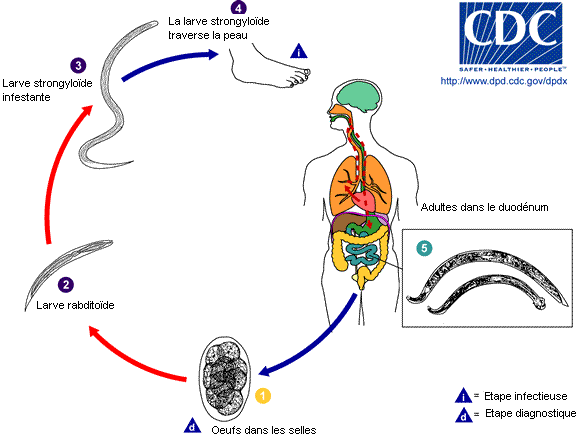
\includegraphics[width=0.4\textwidth,height=\textheight]{Hookworm_LifeCycle.png}
\caption{Cycle parasitaire de l'ankylostome, par CDC - Department of
Parasitic Diseases - Domaine public}
\end{figure}

\newpage

\section{I. Lecture des données et
vérification}\label{i.-lecture-des-donnuxe9es-et-vuxe9rification}

A travers le tableau suivant, voici un récapitulatif de nos données:

\begin{longtable}[]{@{}
  >{\raggedright\arraybackslash}p{(\columnwidth - 4\tabcolsep) * \real{0.2740}}
  >{\raggedright\arraybackslash}p{(\columnwidth - 4\tabcolsep) * \real{0.1096}}
  >{\raggedright\arraybackslash}p{(\columnwidth - 4\tabcolsep) * \real{0.6164}}@{}}
\toprule\noalign{}
\begin{minipage}[b]{\linewidth}\raggedright
Nom de la variable
\end{minipage} & \begin{minipage}[b]{\linewidth}\raggedright
Type
\end{minipage} & \begin{minipage}[b]{\linewidth}\raggedright
Modalités ou exemples de modalités
\end{minipage} \\
\midrule\noalign{}
\endhead
\bottomrule\noalign{}
\endlastfoot
id & int & 440, 336, 60, \ldots{} \\
age & int & 2, 3, 4, 5, 6, 7, 8, 9, 10, 11, 12, \ldots{} \\
agegr & chr & \textless15 yrs, 15-59 yrs, 60+ yrs \\
zone & chr & Nord, Ouest, Sud, Est \\
sexe & int & 0 (masculin ?), 1 (féminin ?) \\
chaussures & chr & ``no'', ``yes'' \\
nb.oeufs & int & 0, 46, 184, 989, 1150, 690, \ldots{} \\
intensite & chr & 0, ``{[}1;1.999{]}'', ``{[}2;+{]}'' \\
ageclasses & chr & \textless16 ans, 16-49, 49 et plus \\
\end{longtable}

Voici l'allure générale de nos données:

\begin{verbatim}
##    id age   agegr  zone sexe chaussures nb.oeufs   intensite ageclasses
## 1 440   2 <15 yrs  Nord    0         no        0           0    <16 ans
## 2 336   2 <15 yrs Ouest    1         no       46 "[1;1.999]"    <16 ans
## 3  60   2 <15 yrs  Nord    1         no      184 "[1;1.999]"    <16 ans
## 4 100   2 <15 yrs Ouest    1         no        0           0    <16 ans
## 5 281   2 <15 yrs   Sud    1         no        0           0    <16 ans
## 6  90   2 <15 yrs Ouest    0         no        0           0    <16 ans
\end{verbatim}

\subsection{I.1 Informations concernant les
individus}\label{i.1-informations-concernant-les-individus}

La table de données contient 238 hommes et 399 femmes et ils sont
répartis de la manière suivante selon la zone géographique:

\includegraphics{Projet_biostatistiques_Ankylostome_files/figure-latex/unnamed-chunk-4-1.pdf}

Regardons les catégories d'âges. Trois variables sont à notre
disposition: age, agegr et ageclasses.

Concernant la variable \textbf{age}:

\begin{longtable}[]{@{}ll@{}}
\toprule\noalign{}
Statistique & Valeur \\
\midrule\noalign{}
\endhead
\bottomrule\noalign{}
\endlastfoot
Min. & 2.00 \\
1st Qu. & 9.00 \\
Median & 23.00 \\
Mean & 25.94 \\
3rd Qu. & 40.00 \\
Max. & 78.00 \\
\end{longtable}

Concernant la variable \textbf{agegr}:

\begin{longtable}[]{@{}ll@{}}
\toprule\noalign{}
Catégorie & Valeur \\
\midrule\noalign{}
\endhead
\bottomrule\noalign{}
\endlastfoot
\textless15 yrs & 259 \\
15-59 yrs & 331 \\
60+ yrs & 47 \\
\end{longtable}

Concernant la variable \textbf{ageclasses}:

\begin{longtable}[]{@{}ll@{}}
\toprule\noalign{}
Catégorie & Valeur \\
\midrule\noalign{}
\endhead
\bottomrule\noalign{}
\endlastfoot
\textless16 ans & 259 \\
16-49 ans & 331 \\
49 et plus & 47 \\
\end{longtable}

\subsection{I.2 Création de la variable ``malade'' et
observations}\label{i.2-cruxe9ation-de-la-variable-malade-et-observations}

Afin de réaliser notre étude, nous créons la variable \textbf{malade}.
Nous considérons qu'un individu est infecté si la variable
\textbf{nb.oeufs} est supérieur à 0. La variable malade vaudra 0 si la
variable \textbf{nb.oeufs} est égal à 0, sinon elle vaudra 1.

Suite à cette création nous constatons qu'il y a 197 personnes non
malades (31\% de l'échantillon) et 440 personnes malades (69\% de
l'échantillon), pour un total de 637 personnes.

\subsection{I.3 Quelques analyses préliminaires
\ldots{}}\label{i.3-quelques-analyses-pruxe9liminaires}

\subsubsection{I.3.a \ldots via des
graphiques}\label{i.3.a-via-des-graphiques}

\subsection{I.3 Quelques analyses préliminaires via des
graphiques}\label{i.3-quelques-analyses-pruxe9liminaires-via-des-graphiques}

La répartition des sexes par zone géographique selon le porte de
chaussures :

\begin{center}\includegraphics{Projet_biostatistiques_Ankylostome_files/figure-latex/unnamed-chunk-7-1} \end{center}

La répartition des personnes porte des chaussures selon l'âge par zone
géographique :

\begin{center}\includegraphics{Projet_biostatistiques_Ankylostome_files/figure-latex/unnamed-chunk-8-1} \end{center}

La répartition des sexes par zone géographique selon l'infection:

\begin{center}\includegraphics{Projet_biostatistiques_Ankylostome_files/figure-latex/unnamed-chunk-9-1} \end{center}

La répartition des personnes infectées et le port de chaussures:

\begin{center}\includegraphics{Projet_biostatistiques_Ankylostome_files/figure-latex/unnamed-chunk-10-1} \end{center}

La répartition des personnes infectées selon leur âge. Pour cela nous
allons créer une nouvelle variable age\_categ car les deux autres
variables qui classent les âges ne nous semblent pas représentatives.
Voici les tranches choisies: \newline - 0 à 5 ans exclus, \newline - 5
ans à 10 ans exclus, \newline - 10 ans à 18 ans exclus, \newline - 19
ans à 30 ans exclus, \newline - 30 à 60 ans exlus, \newline - les plus
de 60 ans

\begin{center}\includegraphics{Projet_biostatistiques_Ankylostome_files/figure-latex/unnamed-chunk-11-1} \end{center}

\subsubsection{I.3.b \ldots via le test du
khi-deux}\label{i.3.b-via-le-test-du-khi-deux}

Le \(\chi^2\) permet de vérifier une relation entre deux variables
qualitatives et de comparer des répartitions d'effectifs. Nous allons
réaliser un text du khi-deux d'homogénéité et d'indépendance.

De plus, nous restons vigilants à la contrainte suivante : 80\% des
effectifs doivent être supérieurs à 5 individus.

Nous testons l'hypothèse nulle H0, les deux variables sont indépendantes
contre H1, il existe une relation entre les deux variables testées.

Dans un premier temps, nous réaliserons ce test avec \emph{zone} en tant
que variable cible, avec \emph{chaussures}, \emph{age\_categ} et
\emph{sexe}. Ensuite, nous réaliserons ce test entre \emph{age\_categ}
et \emph{chaussures}, \emph{age\_categ} et \emph{sexe},
\emph{chaussures} et \emph{sexe}.

\begin{table}[!t]
\caption*{
{\large Test du khi-deux} \\ 
{\small Analyse des relations entre variables}
} 
\fontsize{12.0pt}{14.4pt}\selectfont
\begin{tabular*}{\linewidth}{@{\extracolsep{\fill}}llrl}
\toprule
variable\_cible & variable\_testee & p\_valeur & interpretation \\ 
\midrule\addlinespace[2.5pt]
zone & chaussures & 0.4378 & Indépendance entre zone et chaussures \\ 
zone & ageclasses & 0.9627 & Indépendance entre zone et ageclasses \\ 
zone & sexe & 0.4234 & Indépendance entre zone et sexe \\ 
ageclasses & chaussures & 0.0000 & Dépendance entre ageclasses et chaussures \\ 
ageclasses & sexe & 0.0000 & Dépendance entre ageclasses et sexe \\ 
chaussures & sexe & 0.0000 & Dépendance entre chaussures et sexe \\ 
\bottomrule
\end{tabular*}
\end{table}

\section{II. Modèles}\label{ii.-moduxe8les}

\subsection{II.1 Modèles logistiques avec une variable
qualitative}\label{ii.1-moduxe8les-logistiques-avec-une-variable-qualitative}

La variable cible est \emph{malade}, variable binaire où 1 représente
une infection et 0 une absence d'infection.

Tout d'abord, nous allons regarder différents modèles logistiques selon
seulement une variable qualitative: chaussures ; age ; sexe.

Nous choisirons dans chaque variable, la modalité de référence comme la
modalité la plus réprésentée dans l'échantillon afin d'obtenir une
diminution de la variance des estimateurs.

\subsubsection{Variable chaussures}\label{variable-chaussures}

\begin{verbatim}
## 
##  no yes 
## 385 252
\end{verbatim}

Les modalités possibles de la variable \emph{chaussures} sont
\textbf{no} ou \textbf{yes}. La modalité ``no'' représente 385
observations et ``yes'' 252 observations. Ainsi la modalité de référence
déclarée sera ``yes'' et voici le modèle considéré :

\[malade = \beta_{0} + \beta_{chaussuresno} * chaussuresno \]

\begin{Shaded}
\begin{Highlighting}[]
\DocumentationTok{\#\#\# MODELE DE REGRESSION {-} VAR chaussures }\AlertTok{\#\#\#}
\NormalTok{res\_chaussures }\OtherTok{\textless{}{-}} \FunctionTok{glm}\NormalTok{(malade }\SpecialCharTok{\textasciitilde{}}\NormalTok{ chaussures, }\AttributeTok{family=}\StringTok{"binomial"}\NormalTok{, }\AttributeTok{data=}\NormalTok{data)}
\NormalTok{res\_chaussures}
\end{Highlighting}
\end{Shaded}

\begin{verbatim}
## 
## Call:  glm(formula = malade ~ chaussures, family = "binomial", data = data)
## 
## Coefficients:
##  (Intercept)  chaussuresno  
##       0.6753        0.2156  
## 
## Degrees of Freedom: 636 Total (i.e. Null);  635 Residual
## Null Deviance:       788 
## Residual Deviance: 786.5     AIC: 790.5
\end{verbatim}

\begin{Shaded}
\begin{Highlighting}[]
\FunctionTok{confint}\NormalTok{(res\_chaussures, }\AttributeTok{level=}\FloatTok{0.95}\NormalTok{)}
\end{Highlighting}
\end{Shaded}

\begin{verbatim}
## Waiting for profiling to be done...
\end{verbatim}

\begin{verbatim}
##                   2.5 %    97.5 %
## (Intercept)   0.4175228 0.9405830
## chaussuresno -0.1268667 0.5565847
\end{verbatim}

Nous obtenons \(\beta_{chaussuresno}=0.2156\) et
\(IC_{95%} = [-0.1268667, 0.5565847]
\). Le groupe de référence est représenté par la modélité ``yes''. Ainsi
la valeur obtenue pour
\(\beta_{chaussuresno} - \beta_{chaussuresyes} = ln(\frac{odds(malade=1|chaussures ="no")}{odds(malade=1|chaussures="yes")})\)
est 0.2156, soit :

\[\frac{odds(malade=1|chaussures="no")}{odds(malade=1|chaussures="yes")}= \exp(0.2156) = 1.24\]
Nous pouvons dire que la sous-population des personnes ne portant pas de
chaussures a 1.24 fois plus de chance d'infection que la sous-population
portant des chaussures. L'intervalle de confiance obtenue contient 0 et
est large, il est difficile de conclure en raison de son imprécision.

\subsubsection{Variable sexe}\label{variable-sexe}

\begin{verbatim}
## 
##   0   1 
## 238 399
\end{verbatim}

Les modalités possibles de la variable \emph{sexe} sont \textbf{O} ou
\textbf{1}. La modalité ``0'' (homme) représente 238 observations et
``1''(femme) 399 observations. Ainsi la modalité de référence déclarée
sera ``1'' et voici le modèle considéré :

\[malade = \beta_{0} + \beta_{sexe0} * sexe0 \]

\begin{Shaded}
\begin{Highlighting}[]
\DocumentationTok{\#\#\# MODELE DE REGRESSION {-} VAR chaussures }\AlertTok{\#\#\#}
\NormalTok{res\_sexe }\OtherTok{\textless{}{-}} \FunctionTok{glm}\NormalTok{(malade }\SpecialCharTok{\textasciitilde{}}\NormalTok{ sexe, }\AttributeTok{family=}\StringTok{"binomial"}\NormalTok{, }\AttributeTok{data=}\NormalTok{data)}
\NormalTok{res\_sexe}
\end{Highlighting}
\end{Shaded}

\begin{verbatim}
## 
## Call:  glm(formula = malade ~ sexe, family = "binomial", data = data)
## 
## Coefficients:
## (Intercept)        sexe0  
##      0.8797      -0.1992  
## 
## Degrees of Freedom: 636 Total (i.e. Null);  635 Residual
## Null Deviance:       788 
## Residual Deviance: 786.7     AIC: 790.7
\end{verbatim}

\begin{Shaded}
\begin{Highlighting}[]
\FunctionTok{confint}\NormalTok{(res\_sexe, }\AttributeTok{level=}\FloatTok{0.95}\NormalTok{)}
\end{Highlighting}
\end{Shaded}

\begin{verbatim}
## Waiting for profiling to be done...
\end{verbatim}

\begin{verbatim}
##                  2.5 %    97.5 %
## (Intercept)  0.6671876 1.0986994
## sexe0       -0.5429823 0.1469779
\end{verbatim}

Nous obtenons \$\beta\_\{sexe0\}=-0.1992 \$ et
\(IC_{95%} = [-0.5429823, 0.1469779]
\). Le groupe de référence est représenté par la modélité ``1''(femme).
Ainsi la valeur obtenue pour
\(\beta_{sexe0} - \beta_{sexe1} = ln(\frac{odds(malade=1|sexe ="0")}{odds(malade=1|sexe="1")})\)
est 0.2156, soit :

\[\frac{odds(malade=1|sexe="0")}{odds(malade=1|sexe="1")}= \exp(-0.1992) = 0.82\]
Nous pouvons dire que la sous-population des hommes a 0.82 fois plus de
chance d'infection que la sous-population représentant les femmes, soit
que les hommes ont moins de chance d'être infectés. L'intervalle de
confiance obtenue contient 0 et est large, il est difficile de conclure
en raison de son imprécision.

\section{III. Prédictions}\label{iii.-pruxe9dictions}

\begin{Shaded}
\begin{Highlighting}[]
\DocumentationTok{\#\#\# PREDICTIONS }\AlertTok{\#\#\#}
\CommentTok{\# vect\_estimations \textless{}{-} round(res$fitted.values)}
\CommentTok{\# }
\CommentTok{\# \#Effectif}
\CommentTok{\# tab=table(data$malade, vect\_estimations)}
\CommentTok{\# tab}
\CommentTok{\# }
\CommentTok{\# \#Proportion de personnes pour laquelle la prédiction a été mauvaise: 197 (1 + 196)}
\CommentTok{\# \#1. =\textgreater{} 31\%}
\CommentTok{\# (tab[1,2] + tab[2,1])}
\CommentTok{\# (tab[1,2] + tab[2,1])/sum(tab)}
\CommentTok{\# }
\CommentTok{\# \#2. Proportion de personnes infectées pour laquelle la prédiction était non infecté: 31\% (faux positifs)}
\CommentTok{\# tab[1,2]/sum(tab[,2])}
\CommentTok{\# }
\CommentTok{\# \#3. Proportion de personnes non infectées pour laquelle la prédiction était infectées =\textgreater{} 50\% (faux négatifs)}
\CommentTok{\# tab[2,1]/sum(tab[,1])}
\end{Highlighting}
\end{Shaded}

\subsection{II.2 Modèles logistiques avec plus d'une variable
qualitative}\label{ii.2-moduxe8les-logistiques-avec-plus-dune-variable-qualitative}

\subsubsection{Relations entre les variables
:}\label{relations-entre-les-variables}

chaussures et ageclasses : p = 0.0000

Il y a une relation significative entre le port de chaussures et les
classes d'âge. Cela suggère que l'effet du port de chaussures sur la
probabilité d'être malade pourrait dépendre de l'âge.

ageclasses et sexe : p = 0.0000

Il y a une relation significative entre les classes d'âge et le sexe.
Cela signifie que la distribution des classes d'âge varie selon le sexe.

chaussures et sexe : p = 0.0000

Il y a une relation significative entre le port de chaussures et le
sexe. Cela suggère que le port de chaussures pourrait varier selon le
sexe.

\subsubsection{Ces relations significatives indiquent que
:}\label{ces-relations-significatives-indiquent-que}

Les variables chaussures, ageclasses et sexe ne sont pas indépendantes.

Il est important de considérer les interactions entre ces variables dans
le modèle GLM pour capturer leurs effets combinés.

\subsection{Option 1 : Modèle avec interactions entre port de chaussures
et l'e sexe'age
:}\label{option-1-moduxe8le-avec-interactions-entre-port-de-chaussures-et-le-sexeage}

\[
\text{malade} = \beta_{0} + \beta_{chaussuresno} \text{chaussuresno} + \beta_{16-49} \text{ageclasses}_{16-49} + \beta_{49+} \text{ageclasses}_{49+} + \beta_1 (\text{chaussuresno} \times \text{ageclasses}_{16-49}) + \beta_2 (\text{chaussuresno} \times \text{ageclasses}_{49+})
\]

\begin{Shaded}
\begin{Highlighting}[]
\NormalTok{res\_cha.age }\OtherTok{\textless{}{-}} \FunctionTok{glm}\NormalTok{(malade }\SpecialCharTok{\textasciitilde{}}\NormalTok{ chaussures}\SpecialCharTok{*}\NormalTok{ageclasses, }\AttributeTok{family=}\StringTok{"binomial"}\NormalTok{, }\AttributeTok{data=}\NormalTok{data)}
\NormalTok{res\_cha.age}
\end{Highlighting}
\end{Shaded}

\begin{verbatim}
## 
## Call:  glm(formula = malade ~ chaussures * ageclasses, family = "binomial", 
##     data = data)
## 
## Coefficients:
##                       (Intercept)                       chaussuresno  
##                           0.61310                           -0.19260  
##                   ageclasses16-49               ageclasses49 et plus  
##                           0.07244                            0.08004  
##      chaussuresno:ageclasses16-49  chaussuresno:ageclasses49 et plus  
##                           1.24753                            1.33204  
## 
## Degrees of Freedom: 636 Total (i.e. Null);  631 Residual
## Null Deviance:       788 
## Residual Deviance: 756.5     AIC: 768.5
\end{verbatim}

\begin{Shaded}
\begin{Highlighting}[]
\FunctionTok{confint}\NormalTok{(res\_cha.age, }\AttributeTok{level=}\FloatTok{0.95}\NormalTok{)}
\end{Highlighting}
\end{Shaded}

\begin{verbatim}
## Waiting for profiling to be done...
\end{verbatim}

\begin{verbatim}
##                                         2.5 %    97.5 %
## (Intercept)                       -0.04562779 1.3175075
## chaussuresno                      -0.94419508 0.5200309
## ageclasses16-49                   -0.68845103 0.7962925
## ageclasses49 et plus              -1.09433528 1.3154381
## chaussuresno:ageclasses16-49       0.34583228 2.1867747
## chaussuresno:ageclasses49 et plus -0.26044977 3.0114739
\end{verbatim}

\subsubsection{1. Coefficients du
modèle}\label{coefficients-du-moduxe8le}

Les coefficients indiquent l'effet de chaque variable sur la probabilité
d'être malade (en log-odds). Une valeur positive augmente la
probabilité, tandis qu'une valeur négative la diminue.

\begin{itemize}
\item
  (Intercept) : 0.61310 C'est la valeur de référence (log-odds) lorsque
  toutes les variables sont à leur niveau de référence ( chaussures =
  yes, ageclasses = moins de 16 ans).
\item
  chaussuresno : -0.19260
\end{itemize}

Le fait de ne pas porter de chaussures (chaussures = no) diminue
légèrement les log-odds d'être malade par rapport au port de chaussules,
mais cet effet n'est pas significatif (l'intervalle de confiance à 95 \%
inclut 0).

\begin{itemize}
\tightlist
\item
  ageclasses16-49 : 0.07244
\end{itemize}

Les personnes âgées de 16 à 49 ans ont des log-odds légèrement plus
élevés d'être malades que celles de moins de 16 ans, mais cet effet
n'est pas significatif.

\begin{itemize}
\tightlist
\item
  ageclasses49 et plus : 0.08004
\end{itemize}

Les personnes de 49 ans et plus ont des log-odds légèrement plus élevés
d'être malades que celles de moins de 16 ans, mais cet effet n'est pas
significatif.

\begin{itemize}
\tightlist
\item
  chaussuresno:ageclasses16-49 : 1.24753
\end{itemize}

Il y a une interaction positive et significative entre le fait de ne pas
porter de chaussures et la classe d'âge 16-49 ans. Cela signifie que,
pour cette tranche d'âge, ne pas porter de chaussures augmente
significativement les log-odds d'être malade.

\begin{itemize}
\tightlist
\item
  chaussuresno:ageclasses49 et plus : 1.33204
\end{itemize}

Il y a également une interaction positive entre le fait de ne pas porter
de chaussures et la classe d'âge 49 ans et plus., mais cet effet n'est
pas significatif.

\subsubsection{Conclusion du modèle :}\label{conclusion-du-moduxe8le}

L'interaction entre chaussuresno et ageclasses16-49 est significative,
ce qui suggère que l'effet du port de chaussures sur la probabilité
d'être malade dépend de l'âge pour cette tranche d'âge.

Pour ageclasses49 et plus, l'interaction n'est pas significative, mais
la valeur estimée est élevée (1.33204) avec un intervalle de confiance
large. Cela pourrait indiquer un manque de puissance statistique due à
un échantillon insuffisant dans cette tranche d'âge.

Un modèle simplifié pourrait inclure uniquement l'interaction
significative (chaussuresno:ageclasses16-49)

\subsection{Option 2 : Modèle avec interactions entre port de chaussures
et le sexe
:}\label{option-2-moduxe8le-avec-interactions-entre-port-de-chaussures-et-le-sexe}

\[
\text{malade} = \beta_{0} + \beta_{\text{chaussuresno}} \cdot \text{chaussuresno} + \beta_{\text{sexe0}} \cdot \text{Sexe}_{0} + \beta_{\text{interaction}} \cdot (\text{chaussuresno} \times \text{Sexe}_{0})
\]

\begin{Shaded}
\begin{Highlighting}[]
\NormalTok{res\_cha.sex }\OtherTok{\textless{}{-}} \FunctionTok{glm}\NormalTok{(malade }\SpecialCharTok{\textasciitilde{}}\NormalTok{ chaussures}\SpecialCharTok{*}\NormalTok{sexe, }\AttributeTok{family=}\StringTok{"binomial"}\NormalTok{, }\AttributeTok{data=}\NormalTok{data)}
\NormalTok{res\_cha.sex}
\end{Highlighting}
\end{Shaded}

\begin{verbatim}
## 
## Call:  glm(formula = malade ~ chaussures * sexe, family = "binomial", 
##     data = data)
## 
## Coefficients:
##        (Intercept)        chaussuresno               sexe0  chaussuresno:sexe0  
##            0.83130             0.06252            -0.23778             0.22321  
## 
## Degrees of Freedom: 636 Total (i.e. Null);  633 Residual
## Null Deviance:       788 
## Residual Deviance: 785.7     AIC: 793.7
\end{verbatim}

\begin{Shaded}
\begin{Highlighting}[]
\FunctionTok{confint}\NormalTok{(res\_cha.sex, }\AttributeTok{level=}\FloatTok{0.95}\NormalTok{)}
\end{Highlighting}
\end{Shaded}

\begin{verbatim}
## Waiting for profiling to be done...
\end{verbatim}

\begin{verbatim}
##                         2.5 %    97.5 %
## (Intercept)         0.3908125 1.2987157
## chaussuresno       -0.4627775 0.5688407
## sexe0              -0.8007575 0.3105208
## chaussuresno:sexe0 -0.5517709 1.0184625
\end{verbatim}

\subsection{1. Coefficients du
modèle}\label{coefficients-du-moduxe8le-1}

*(Intercept) : 0.83130

C'est la valeur de référence (log-odds) lorsque toutes les variables
sont à leur niveau de référence(chaussures = yes,sexe = 1 les hommes). )

\begin{itemize}
\tightlist
\item
  chaussuresno : 0.06252
\end{itemize}

Le fait de ne pas porter de chaussures (chaussures = no) augmente
légèrement les log-odds d'être malade par rapport au port de chaussures,
mais cet effet n'est pas significatif (l'intervalle de confiance à 95 \%
inclut 0).

\begin{itemize}
\tightlist
\item
  sexe0 : -0.23778
\end{itemize}

Le sexe de référence sexe = 0 (les femmes) a des log-odds légèrement
plus faibles d'être malade que le sexe de référence sexe = 1, mais cet
effet n'est pas significatif.

\begin{itemize}
\tightlist
\item
  chaussuresno:sexe0 : 0.22321
\end{itemize}

Il y a une interaction positive entre le fait de ne pas porter de
chaussures et le sexe sexe = 0. Cela signifie que, pour le sexe sexe =
0, ne pas porter de chaussures augmente légèrement les log-odds d'être
malade. Cependant, cet effet n'est pas significatif.

\subsubsection{conclusion :}\label{conclusion}

le modèle n'identifie aucun effet significatif des variables
explicatives (chaussures, sexe et leur interaction) sur la variable
cible (malade)

\subsection{Option 3 : Modèle avec interactions entre port de chaussures
et sexe avec l'effet additif d'age
:}\label{option-3-moduxe8le-avec-interactions-entre-port-de-chaussures-et-sexe-avec-leffet-additif-dage}

\[
\text{malade} = \beta_{0} + \beta_{\text{chaussuresno}} \cdot \text{chaussuresno} + \beta_{\text{sexe0}} \cdot \text{Sexe}_{0} + \beta_{\text{ageclasses16-49}} \cdot \text{ageclasses16-49} + \beta_{\text{ageclasses49 et plus}} \cdot \text{ageclasses49 et plus} + \beta_{\text{interaction}} \cdot (\text{chaussuresno} \times \text{Sexe}_{0})
\]

\begin{Shaded}
\begin{Highlighting}[]
\NormalTok{res\_cha.age\_sex }\OtherTok{\textless{}{-}} \FunctionTok{glm}\NormalTok{(malade }\SpecialCharTok{\textasciitilde{}}\NormalTok{ chaussures}\SpecialCharTok{*}\NormalTok{ageclasses }\SpecialCharTok{+}\NormalTok{ sexe, }\AttributeTok{family=}\StringTok{"binomial"}\NormalTok{, }\AttributeTok{data=}\NormalTok{data)}
\NormalTok{res\_cha.age\_sex}
\end{Highlighting}
\end{Shaded}

\begin{verbatim}
## 
## Call:  glm(formula = malade ~ chaussures * ageclasses + sexe, family = "binomial", 
##     data = data)
## 
## Coefficients:
##                       (Intercept)                       chaussuresno  
##                           0.72396                           -0.27201  
##                   ageclasses16-49               ageclasses49 et plus  
##                           0.08015                            0.05876  
##                             sexe0       chaussuresno:ageclasses16-49  
##                          -0.17655                            1.25254  
## chaussuresno:ageclasses49 et plus  
##                           1.34759  
## 
## Degrees of Freedom: 636 Total (i.e. Null);  630 Residual
## Null Deviance:       788 
## Residual Deviance: 755.7     AIC: 769.7
\end{verbatim}

\begin{Shaded}
\begin{Highlighting}[]
\FunctionTok{confint}\NormalTok{(res\_cha.age\_sex, }\AttributeTok{level=}\FloatTok{0.95}\NormalTok{)}
\end{Highlighting}
\end{Shaded}

\begin{verbatim}
## Waiting for profiling to be done...
\end{verbatim}

\begin{verbatim}
##                                         2.5 %    97.5 %
## (Intercept)                        0.01824004 1.4726839
## chaussuresno                      -1.04575335 0.4634776
## ageclasses16-49                   -0.68143990 0.8049178
## ageclasses49 et plus              -1.11782714 1.2958217
## sexe0                             -0.57614423 0.2236899
## chaussuresno:ageclasses16-49       0.35012245 2.1925361
## chaussuresno:ageclasses49 et plus -0.24618336 3.0283592
\end{verbatim}

\subsubsection{Coefficients du
modèle}\label{coefficients-du-moduxe8le-2}

\begin{itemize}
\tightlist
\item
  ageclasses16-49 : 0.91803
\end{itemize}

Les personnes âgées de 16 à 49 ans ont des log-odds significativement
plus élevés d'être malades que celles de moins de 16 ans (la classe de
référence).

\begin{itemize}
\tightlist
\item
  ageclasses49 et plus : 1.02286
\end{itemize}

Les personnes de 49 ans et plus ont des log-odds significativement plus
élevés d'être malades que celles de moins de 16 ans (la classe de
référence).

\begin{itemize}
\tightlist
\item
  les autre coefficient sont non significatifs.
\end{itemize}

cha* sexe + age : AIC: 775.6, cha* age + sexe : 769.7, sexe\emph{age
+chau : AIC: 776.9 cha} age :AIC: 768.5, cha* sexe : AIC: 793.7

\begin{longtable}[]{@{}ll@{}}
\toprule\noalign{}
Modèls & AIC \\
\midrule\noalign{}
\endhead
\bottomrule\noalign{}
\endlastfoot
cha* sexe + age & 775.6 \\
cha* age + sexe & 769.7 \\
sexe*age +chau & 776.9 \\
cha* age & 768.5 \\
cha* sexe & 793.7 \\
\end{longtable}

Selon le critère AIC, le meilleur modèle pour prédire la maladie est
celui incluant l'interaction entre chaussures et âge (cha*age), car il
présente la plus faible valeur d'AIC (768.5).

\section{Conclusion}\label{conclusion-1}

A MODIFIER

Il est important de noter que pour prévenir la population de ce type
d'infection, il vaut mieux éviter de marcher pieds nus, d'utiliser des
eaux usées et de bien utiliser des dispositifs de toilettes, d'hygiène
pour éviter la présence de selles au sol. Le diagnostic de l'infection
peut-être réalisé via un examen d'un échantillon de selles ou d'analyse
de sang. \newpage 

\section{Annexe Code R}\label{annexe-code-r}

\begin{Shaded}
\begin{Highlighting}[]
\NormalTok{knitr}\SpecialCharTok{::}\NormalTok{opts\_chunk}\SpecialCharTok{$}\FunctionTok{set}\NormalTok{(}\AttributeTok{echo =} \ConstantTok{TRUE}\NormalTok{)}
\DocumentationTok{\#\#\# LIBRAIRIES UTILISEES }\AlertTok{\#\#\#}
\FunctionTok{library}\NormalTok{(dplyr)}
\FunctionTok{library}\NormalTok{(ggplot2)}
\FunctionTok{library}\NormalTok{(gt)}
\DocumentationTok{\#\#\# LECTURE DES DONNEES ET MODALITES }\AlertTok{\#\#\#}
\NormalTok{data }\OtherTok{\textless{}{-}} \FunctionTok{read.csv}\NormalTok{(}\StringTok{"Ankylostome.csv"}\NormalTok{)}
\NormalTok{data }\OtherTok{\textless{}{-}}\NormalTok{ data }\SpecialCharTok{\%\textgreater{}\%} \FunctionTok{select}\NormalTok{(}\SpecialCharTok{{-}}\FunctionTok{c}\NormalTok{(...}\DecValTok{1}\NormalTok{, X))}

\NormalTok{modalites\_uniques }\OtherTok{\textless{}{-}} \FunctionTok{lapply}\NormalTok{(data, }\ControlFlowTok{function}\NormalTok{(colonne) \{}
\NormalTok{  unique\_values }\OtherTok{\textless{}{-}} \FunctionTok{unique}\NormalTok{(colonne) }
\NormalTok{  count\_values }\OtherTok{\textless{}{-}} \FunctionTok{length}\NormalTok{(unique\_values) }
  \FunctionTok{list}\NormalTok{(}\AttributeTok{Modalites =}\NormalTok{ unique\_values, }\AttributeTok{Nombre =}\NormalTok{ count\_values)}
\NormalTok{\})}

\DocumentationTok{\#\#\# ALLURE GENERALE DES DONNÉES }\AlertTok{\#\#\#}
\FunctionTok{head}\NormalTok{(data)}

\DocumentationTok{\#\#\# SEXE DES INDIVIDUS }\AlertTok{\#\#\#}
\NormalTok{table\_sexe }\OtherTok{\textless{}{-}} \FunctionTok{table}\NormalTok{(data}\SpecialCharTok{$}\NormalTok{sexe)}

\DocumentationTok{\#\#\# REPARTITION SELON LES ZONES }\AlertTok{\#\#\#}
\FunctionTok{ggplot}\NormalTok{(data, }\FunctionTok{aes}\NormalTok{(}\AttributeTok{x =}\NormalTok{ zone, }\AttributeTok{fill =} \FunctionTok{as.factor}\NormalTok{(sexe))) }\SpecialCharTok{+}
  \FunctionTok{geom\_bar}\NormalTok{(}\AttributeTok{position =} \StringTok{"dodge"}\NormalTok{) }\SpecialCharTok{+}
  \FunctionTok{labs}\NormalTok{(}
    \AttributeTok{title =} \StringTok{"Répartition des sexes par zone"}\NormalTok{,}
    \AttributeTok{x =} \StringTok{"Zone"}\NormalTok{,}
    \AttributeTok{y =} \StringTok{"Nombre de personnes"}\NormalTok{,}
    \AttributeTok{fill =} \StringTok{"Sexe"}
\NormalTok{  ) }\SpecialCharTok{+}
  \FunctionTok{scale\_fill\_manual}\NormalTok{(}
    \AttributeTok{values =} \FunctionTok{c}\NormalTok{(}\StringTok{"0"} \OtherTok{=} \StringTok{"blue"}\NormalTok{, }\StringTok{"1"} \OtherTok{=} \StringTok{"pink"}\NormalTok{),}
    \AttributeTok{labels =} \FunctionTok{c}\NormalTok{(}\StringTok{"0"} \OtherTok{=} \StringTok{"Hommes"}\NormalTok{, }\StringTok{"1"} \OtherTok{=} \StringTok{"Femmes"}\NormalTok{)}
\NormalTok{  ) }\SpecialCharTok{+}
  \FunctionTok{theme\_minimal}\NormalTok{()}

\DocumentationTok{\#\#\# AGE DES INDIVIDUS }\AlertTok{\#\#\#}
\NormalTok{age }\OtherTok{\textless{}{-}} \FunctionTok{summary}\NormalTok{(data[}\StringTok{"age"}\NormalTok{])}
\NormalTok{agegr }\OtherTok{\textless{}{-}} \FunctionTok{table}\NormalTok{(data}\SpecialCharTok{$}\NormalTok{agegr)}
\NormalTok{ageclasses }\OtherTok{\textless{}{-}} \FunctionTok{table}\NormalTok{(data}\SpecialCharTok{$}\NormalTok{ageclasses)}

\DocumentationTok{\#\#\# CREATION DE LA VARIABLE MALADE ET OBSERVATIONS }\AlertTok{\#\#\#}
\NormalTok{data }\OtherTok{\textless{}{-}}\NormalTok{ data }\SpecialCharTok{\%\textgreater{}\%} \FunctionTok{mutate}\NormalTok{(}\AttributeTok{malade =} \FunctionTok{ifelse}\NormalTok{(nb.oeufs }\SpecialCharTok{==} \DecValTok{0}\NormalTok{, }\DecValTok{0}\NormalTok{, }\DecValTok{1}\NormalTok{))}
\NormalTok{malades }\OtherTok{\textless{}{-}} \FunctionTok{table}\NormalTok{(data}\SpecialCharTok{$}\NormalTok{malade)}
\NormalTok{pourcentages\_malades }\OtherTok{\textless{}{-}} \FunctionTok{prop.table}\NormalTok{(malades) }\SpecialCharTok{*} \DecValTok{100}

\DocumentationTok{\#\#\# répartition d\textquotesingle{}age par zone géographique selon la variable Sexe }\AlertTok{\#\#\#}
\FunctionTok{ggplot}\NormalTok{(data, }\FunctionTok{aes}\NormalTok{(}\AttributeTok{x =} \FunctionTok{as.factor}\NormalTok{(chaussures), }\AttributeTok{fill =} \FunctionTok{as.factor}\NormalTok{(sexe))) }\SpecialCharTok{+}
  \FunctionTok{geom\_bar}\NormalTok{(}\AttributeTok{position =} \StringTok{"stack"}\NormalTok{) }\SpecialCharTok{+}   
  \FunctionTok{facet\_wrap}\NormalTok{(}\SpecialCharTok{\textasciitilde{}}\NormalTok{ zone) }\SpecialCharTok{+}             
  \FunctionTok{labs}\NormalTok{(}\AttributeTok{title =} \StringTok{"Répartition de sexe selon porte chaussures et zone"}\NormalTok{,}
       \AttributeTok{x =} \StringTok{"Porte Chaussures"}\NormalTok{,}
       \AttributeTok{y =} \StringTok{"Nombre de cas"}\NormalTok{,}
       \AttributeTok{fill =} \StringTok{"Sexe"}\NormalTok{) }\SpecialCharTok{+}   
  \FunctionTok{scale\_fill\_manual}\NormalTok{(}\AttributeTok{values =} \FunctionTok{c}\NormalTok{(}\StringTok{"blue"}\NormalTok{, }\StringTok{"pink"}\NormalTok{)) }\SpecialCharTok{+}  
  \FunctionTok{theme\_minimal}\NormalTok{()  }

\DocumentationTok{\#\#\# répartition du port de chaussures par rapport au classe d\textquotesingle{}age }\AlertTok{\#\#\#}
\FunctionTok{ggplot}\NormalTok{(data, }\FunctionTok{aes}\NormalTok{(}\AttributeTok{x =}\NormalTok{ ageclasses, }\AttributeTok{fill =}\NormalTok{ chaussures)) }\SpecialCharTok{+}
  \FunctionTok{geom\_bar}\NormalTok{(}\AttributeTok{position =} \StringTok{"stack"}\NormalTok{) }\SpecialCharTok{+}   
  \FunctionTok{facet\_wrap}\NormalTok{(}\SpecialCharTok{\textasciitilde{}}\NormalTok{ zone) }\SpecialCharTok{+}
  \FunctionTok{labs}\NormalTok{(}\AttributeTok{title =} \StringTok{"Répartition du port de chaussures selon age"}\NormalTok{,}
       \AttributeTok{x =} \StringTok{"Âge"}\NormalTok{,}
       \AttributeTok{y =} \StringTok{"Nombre de cas"}\NormalTok{,}
       \AttributeTok{fill =} \StringTok{"Type de chaussures"}\NormalTok{) }\SpecialCharTok{+}   
  \FunctionTok{scale\_fill\_manual}\NormalTok{(}\AttributeTok{values =} \FunctionTok{c}\NormalTok{(}\StringTok{"lightblue"}\NormalTok{, }\StringTok{"orange"}\NormalTok{)) }\SpecialCharTok{+}  
  \FunctionTok{theme\_minimal}\NormalTok{()  }

\DocumentationTok{\#\#\# répartition des sexes par zone géographique selon l\textquotesingle{}infection }\AlertTok{\#\#\#}
\FunctionTok{ggplot}\NormalTok{(data, }\FunctionTok{aes}\NormalTok{(}\AttributeTok{x =} \FunctionTok{as.factor}\NormalTok{(sexe), }\AttributeTok{fill =} \FunctionTok{as.factor}\NormalTok{(malade))) }\SpecialCharTok{+}
  \FunctionTok{geom\_bar}\NormalTok{(}\AttributeTok{position =} \StringTok{"stack"}\NormalTok{) }\SpecialCharTok{+}   
  \FunctionTok{facet\_wrap}\NormalTok{(}\SpecialCharTok{\textasciitilde{}}\NormalTok{ zone) }\SpecialCharTok{+}             
  \FunctionTok{labs}\NormalTok{(}\AttributeTok{title =} \StringTok{"Répartition des malades par sexe et zone"}\NormalTok{,}
       \AttributeTok{x =} \StringTok{"Sexe"}\NormalTok{,}
       \AttributeTok{y =} \StringTok{"Nombre de cas"}\NormalTok{,}
       \AttributeTok{fill =} \StringTok{"État de l\textquotesingle{}infection"}\NormalTok{) }\SpecialCharTok{+}   
  \FunctionTok{scale\_fill\_manual}\NormalTok{(}\AttributeTok{values =} \FunctionTok{c}\NormalTok{(}\StringTok{"lightblue"}\NormalTok{, }\StringTok{"orange"}\NormalTok{)) }\SpecialCharTok{+}  
  \FunctionTok{theme\_minimal}\NormalTok{()  }

\DocumentationTok{\#\#\# répartition des personnes infectées et le port de chaussures }\AlertTok{\#\#\#}
\FunctionTok{ggplot}\NormalTok{(data, }\FunctionTok{aes}\NormalTok{(}\AttributeTok{x =}\NormalTok{ chaussures, }\AttributeTok{fill =} \FunctionTok{as.factor}\NormalTok{(malade))) }\SpecialCharTok{+}
  \FunctionTok{geom\_bar}\NormalTok{(}\AttributeTok{position =} \StringTok{"stack"}\NormalTok{) }\SpecialCharTok{+}   
  \FunctionTok{labs}\NormalTok{(}\AttributeTok{title =} \StringTok{"Répartition des personnes infectées selon le port de chaussures"}\NormalTok{,}
       \AttributeTok{x =} \StringTok{"Type de chaussures"}\NormalTok{,}
       \AttributeTok{y =} \StringTok{"Nombre de cas"}\NormalTok{,}
       \AttributeTok{fill =} \StringTok{"État de l\textquotesingle{}infection"}\NormalTok{) }\SpecialCharTok{+}   
  \FunctionTok{scale\_fill\_manual}\NormalTok{(}\AttributeTok{values =} \FunctionTok{c}\NormalTok{(}\StringTok{"lightblue"}\NormalTok{, }\StringTok{"orange"}\NormalTok{)) }\SpecialCharTok{+}  
  \FunctionTok{theme\_minimal}\NormalTok{()  }

\DocumentationTok{\#\#\# CREATION DES CLASSES D\textquotesingle{}AGE ET GRAPHIQUE }\AlertTok{\#\#\#}
\NormalTok{data}\SpecialCharTok{$}\NormalTok{age\_categ }\OtherTok{\textless{}{-}} \FunctionTok{cut}\NormalTok{(data}\SpecialCharTok{$}\NormalTok{age, }
                      \AttributeTok{breaks =} \FunctionTok{c}\NormalTok{(}\DecValTok{0}\NormalTok{, }\DecValTok{5}\NormalTok{, }\DecValTok{10}\NormalTok{, }\DecValTok{18}\NormalTok{, }\DecValTok{30}\NormalTok{, }\DecValTok{60}\NormalTok{, }\ConstantTok{Inf}\NormalTok{), }
                      \AttributeTok{labels =} \FunctionTok{c}\NormalTok{(}\StringTok{"0{-}5 ans"}\NormalTok{, }\StringTok{"5{-}10 ans"}\NormalTok{, }\StringTok{"10{-}18 ans"}\NormalTok{, }\StringTok{"19{-}30 ans"}\NormalTok{, }\StringTok{"30{-}60 ans"}\NormalTok{, }\StringTok{"60+ ans"}\NormalTok{),}
                      \AttributeTok{right =} \ConstantTok{FALSE}\NormalTok{) }

\NormalTok{data\_malade }\OtherTok{\textless{}{-}} \FunctionTok{subset}\NormalTok{(data, malade }\SpecialCharTok{==} \DecValTok{1}\NormalTok{)}

\FunctionTok{ggplot}\NormalTok{(data\_malade, }\FunctionTok{aes}\NormalTok{(}\AttributeTok{x =}\NormalTok{ age\_categ)) }\SpecialCharTok{+}
  \FunctionTok{geom\_bar}\NormalTok{(}\AttributeTok{fill =} \StringTok{"lightblue"}\NormalTok{) }\SpecialCharTok{+}
  \FunctionTok{labs}\NormalTok{(}\AttributeTok{title =} \StringTok{"Répartition des personnes infectées par tranches d\textquotesingle{}âge"}\NormalTok{,}
       \AttributeTok{x =} \StringTok{"Âge"}\NormalTok{,}
       \AttributeTok{y =} \StringTok{"Nombre de personnes infectées"}\NormalTok{) }\SpecialCharTok{+}
  \FunctionTok{theme\_minimal}\NormalTok{()}


\NormalTok{resultat }\OtherTok{\textless{}{-}} \FunctionTok{data.frame}\NormalTok{(}
  \AttributeTok{variable\_cible =} \FunctionTok{character}\NormalTok{(),}
  \AttributeTok{variable\_testee =} \FunctionTok{character}\NormalTok{(),}
  \AttributeTok{p\_valeur =} \FunctionTok{numeric}\NormalTok{(),}
  \AttributeTok{interpretation =} \FunctionTok{character}\NormalTok{())}

\NormalTok{tests }\OtherTok{\textless{}{-}} \FunctionTok{list}\NormalTok{(}
  \FunctionTok{list}\NormalTok{(}\AttributeTok{cible =} \StringTok{"zone"}\NormalTok{, }\AttributeTok{testee =} \StringTok{"chaussures"}\NormalTok{),}
  \FunctionTok{list}\NormalTok{(}\AttributeTok{cible =} \StringTok{"zone"}\NormalTok{, }\AttributeTok{testee =} \StringTok{"ageclasses"}\NormalTok{),}
  \FunctionTok{list}\NormalTok{(}\AttributeTok{cible =} \StringTok{"zone"}\NormalTok{, }\AttributeTok{testee =} \StringTok{"sexe"}\NormalTok{),}
  \FunctionTok{list}\NormalTok{(}\AttributeTok{cible =} \StringTok{"ageclasses"}\NormalTok{, }\AttributeTok{testee =} \StringTok{"chaussures"}\NormalTok{),}
  \FunctionTok{list}\NormalTok{(}\AttributeTok{cible =} \StringTok{"ageclasses"}\NormalTok{, }\AttributeTok{testee =} \StringTok{"sexe"}\NormalTok{),}
  \FunctionTok{list}\NormalTok{(}\AttributeTok{cible =} \StringTok{"chaussures"}\NormalTok{, }\AttributeTok{testee =} \StringTok{"sexe"}\NormalTok{)}
\NormalTok{)}

\ControlFlowTok{for}\NormalTok{ (test }\ControlFlowTok{in}\NormalTok{ tests) \{}
\NormalTok{  cible }\OtherTok{\textless{}{-}}\NormalTok{ test}\SpecialCharTok{$}\NormalTok{cible}
\NormalTok{  testee }\OtherTok{\textless{}{-}}\NormalTok{ test}\SpecialCharTok{$}\NormalTok{testee}
\NormalTok{    table\_contingence }\OtherTok{\textless{}{-}} \FunctionTok{table}\NormalTok{(data[[cible]], data[[testee]])}
  
  \ControlFlowTok{if}\NormalTok{ (}\FunctionTok{any}\NormalTok{(}\FunctionTok{chisq.test}\NormalTok{(table\_contingence)}\SpecialCharTok{$}\NormalTok{expected }\SpecialCharTok{\textless{}} \DecValTok{5}\NormalTok{)) \{}
\NormalTok{    p\_valeur }\OtherTok{\textless{}{-}} \ConstantTok{NA}
\NormalTok{    interpretation }\OtherTok{\textless{}{-}} \StringTok{"Test invalide (effectifs attendus \textless{} 5)"}
\NormalTok{  \} }\ControlFlowTok{else}\NormalTok{ \{}
\NormalTok{    test\_resultat }\OtherTok{\textless{}{-}} \FunctionTok{chisq.test}\NormalTok{(table\_contingence)}
\NormalTok{    p\_valeur }\OtherTok{\textless{}{-}}\NormalTok{ test\_resultat}\SpecialCharTok{$}\NormalTok{p.value}
\NormalTok{    interpretation }\OtherTok{\textless{}{-}} \FunctionTok{ifelse}\NormalTok{(}
\NormalTok{      p\_valeur }\SpecialCharTok{\textless{}} \FloatTok{0.05}\NormalTok{,}
      \FunctionTok{paste}\NormalTok{(}\StringTok{"Dépendance entre"}\NormalTok{, cible, }\StringTok{"et"}\NormalTok{, testee),}
      \FunctionTok{paste}\NormalTok{(}\StringTok{"Indépendance entre"}\NormalTok{, cible, }\StringTok{"et"}\NormalTok{, testee)}
\NormalTok{    )}
\NormalTok{  \}}
  
\NormalTok{  resultat }\OtherTok{\textless{}{-}} \FunctionTok{rbind}\NormalTok{(}
\NormalTok{    resultat,}
    \FunctionTok{data.frame}\NormalTok{(}
      \AttributeTok{variable\_cible =}\NormalTok{ cible,}
      \AttributeTok{variable\_testee =}\NormalTok{ testee,}
      \AttributeTok{p\_valeur =} \FunctionTok{round}\NormalTok{(p\_valeur, }\DecValTok{4}\NormalTok{),}
      \AttributeTok{interpretation =}\NormalTok{ interpretation}
\NormalTok{    )}
\NormalTok{  )}
\NormalTok{\}}

\NormalTok{resultat }\SpecialCharTok{\%\textgreater{}\%}
  \FunctionTok{gt}\NormalTok{() }\SpecialCharTok{\%\textgreater{}\%}
  \FunctionTok{tab\_header}\NormalTok{(}
    \AttributeTok{title =} \StringTok{"Test du khi{-}deux"}\NormalTok{,}
    \AttributeTok{subtitle =} \StringTok{"Analyse des relations entre variables"}
\NormalTok{  ) }

\FunctionTok{table}\NormalTok{(data}\SpecialCharTok{$}\NormalTok{chaussures)}

\NormalTok{data}\SpecialCharTok{$}\NormalTok{chaussures }\OtherTok{\textless{}{-}} \FunctionTok{relevel}\NormalTok{(}\FunctionTok{factor}\NormalTok{(data}\SpecialCharTok{$}\NormalTok{chaussures), }\AttributeTok{ref =} \StringTok{"yes"}\NormalTok{)}
\DocumentationTok{\#\#\# MODELE DE REGRESSION {-} VAR chaussures }\AlertTok{\#\#\#}
\NormalTok{res\_chaussures }\OtherTok{\textless{}{-}} \FunctionTok{glm}\NormalTok{(malade }\SpecialCharTok{\textasciitilde{}}\NormalTok{ chaussures, }\AttributeTok{family=}\StringTok{"binomial"}\NormalTok{, }\AttributeTok{data=}\NormalTok{data)}
\NormalTok{res\_chaussures}
\FunctionTok{confint}\NormalTok{(res\_chaussures, }\AttributeTok{level=}\FloatTok{0.95}\NormalTok{)}
\FunctionTok{table}\NormalTok{(data}\SpecialCharTok{$}\NormalTok{sexe)}

\NormalTok{data}\SpecialCharTok{$}\NormalTok{sexe }\OtherTok{\textless{}{-}} \FunctionTok{relevel}\NormalTok{(}\FunctionTok{factor}\NormalTok{(data}\SpecialCharTok{$}\NormalTok{sexe), }\AttributeTok{ref =} \StringTok{"1"}\NormalTok{)}
\DocumentationTok{\#\#\# MODELE DE REGRESSION {-} VAR chaussures }\AlertTok{\#\#\#}
\NormalTok{res\_sexe }\OtherTok{\textless{}{-}} \FunctionTok{glm}\NormalTok{(malade }\SpecialCharTok{\textasciitilde{}}\NormalTok{ sexe, }\AttributeTok{family=}\StringTok{"binomial"}\NormalTok{, }\AttributeTok{data=}\NormalTok{data)}
\NormalTok{res\_sexe}
\FunctionTok{confint}\NormalTok{(res\_sexe, }\AttributeTok{level=}\FloatTok{0.95}\NormalTok{)}

\DocumentationTok{\#\#\# PREDICTIONS }\AlertTok{\#\#\#}
\CommentTok{\# vect\_estimations \textless{}{-} round(res$fitted.values)}
\CommentTok{\# }
\CommentTok{\# \#Effectif}
\CommentTok{\# tab=table(data$malade, vect\_estimations)}
\CommentTok{\# tab}
\CommentTok{\# }
\CommentTok{\# \#Proportion de personnes pour laquelle la prédiction a été mauvaise: 197 (1 + 196)}
\CommentTok{\# \#1. =\textgreater{} 31\%}
\CommentTok{\# (tab[1,2] + tab[2,1])}
\CommentTok{\# (tab[1,2] + tab[2,1])/sum(tab)}
\CommentTok{\# }
\CommentTok{\# \#2. Proportion de personnes infectées pour laquelle la prédiction était non infecté: 31\% (faux positifs)}
\CommentTok{\# tab[1,2]/sum(tab[,2])}
\CommentTok{\# }
\CommentTok{\# \#3. Proportion de personnes non infectées pour laquelle la prédiction était infectées =\textgreater{} 50\% (faux négatifs)}
\CommentTok{\# tab[2,1]/sum(tab[,1])}

\NormalTok{res\_cha.age }\OtherTok{\textless{}{-}} \FunctionTok{glm}\NormalTok{(malade }\SpecialCharTok{\textasciitilde{}}\NormalTok{ chaussures}\SpecialCharTok{*}\NormalTok{ageclasses, }\AttributeTok{family=}\StringTok{"binomial"}\NormalTok{, }\AttributeTok{data=}\NormalTok{data)}
\NormalTok{res\_cha.age}
\FunctionTok{confint}\NormalTok{(res\_cha.age, }\AttributeTok{level=}\FloatTok{0.95}\NormalTok{)}
\NormalTok{res\_cha.sex }\OtherTok{\textless{}{-}} \FunctionTok{glm}\NormalTok{(malade }\SpecialCharTok{\textasciitilde{}}\NormalTok{ chaussures}\SpecialCharTok{*}\NormalTok{sexe, }\AttributeTok{family=}\StringTok{"binomial"}\NormalTok{, }\AttributeTok{data=}\NormalTok{data)}
\NormalTok{res\_cha.sex}
\FunctionTok{confint}\NormalTok{(res\_cha.sex, }\AttributeTok{level=}\FloatTok{0.95}\NormalTok{)}
\NormalTok{res\_cha.age\_sex }\OtherTok{\textless{}{-}} \FunctionTok{glm}\NormalTok{(malade }\SpecialCharTok{\textasciitilde{}}\NormalTok{ chaussures}\SpecialCharTok{*}\NormalTok{ageclasses }\SpecialCharTok{+}\NormalTok{ sexe, }\AttributeTok{family=}\StringTok{"binomial"}\NormalTok{, }\AttributeTok{data=}\NormalTok{data)}
\NormalTok{res\_cha.age\_sex}
\FunctionTok{confint}\NormalTok{(res\_cha.age\_sex, }\AttributeTok{level=}\FloatTok{0.95}\NormalTok{)}
\end{Highlighting}
\end{Shaded}


\end{document}
